\documentclass{article}
\usepackage{graphicx}
\usepackage[margin=1.5cm]{geometry}
\usepackage{amsmath}

\begin{document}
\twocolumn

\title{Tuesday Warm Up, Unit 2: Applications}
\author{Prof. Jordan C. Hanson}
\maketitle

\section{Memory Bank}

\begin{enumerate}
\item \textbf{Human optical receptor cells}.  \textit{Rods} and \textit{cones} detect low-sensitivity light and color, respectively.  There are three cone types: red, green, and blue sensitive.
\item \textbf{Hexadecimal representation}.  A \textit{hexadecimal} number uses digits from 0-9, and then A to F, to represent the numbers 0-15.  A two-digit hexadecimal number has multiples of $16^{1}$ in the first digit, followed by multiples of $16^{0} = 1$ in the second digit.  For example, $F9$ is $15 \times 16^1 + 9 \times 16^0$, or $240 + 9 = 249$.
\item \textbf{RGB Color Coding}.  Amounts of red, green, and blue in a signal can be encoded each with a number between 0 and 255 (8 bits).  Since $FF$ in hexadecimal represents $15 \times 16^1 + 15 = 240+15=255$, red, blue, and green can each be represented by a two-digit hexadecimal number.  The color code $00$ represents no brightness, and FF represents maximum brightness.  For example, 000000 represents no red, no blue, and no green, so black.  Also, 00FF00 represents pure blue, and FFFF00 represents purple.
\item \textbf{Charge Coupled Device (CCD)}.  A device that samples and digitizes optical images.
\end{enumerate}

\section{Image Formation and Display}

\begin{enumerate}
\item (a) Consider one pixel within an image.  It has a color code 99CC99, a kind of blue-gray.  There is one byte (8 bits) per color.  How many bits per pixel? (b) If this pixel is part of a 256 by 256 pixel image, how many bits are there, total, in the color image? (c) If one such image forms part of a video stream, at 30 images per second (to align with human perception), what is the total data rate? \\ \vspace{2.5cm}
\item Suppose we convert the video stream in the previous exercise to black and white style, with just 8 bits per pixel representing black (00) to white (FF).  What is the new data rate? \\ \vspace{2cm}
\item Consider now a 128 by 128 pixel CCD (Fig. \ref{fig:2}) with only black and white sensitivity.  (a) If we want 30 frames per second (fps), what is the total data rate? (b) Each row must be read before the next, converting the entire image into a serial data stream.  At what rate must we read each row?
\end{enumerate}

\begin{figure}
\centering
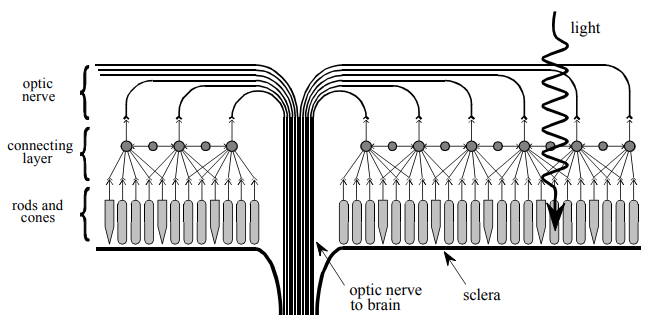
\includegraphics[width=0.35\textwidth]{optic_nerve.png}
\caption{\label{fig:1} The optic nerve system within the human eye. (Top layer) The optic nerve is comprised of fibers that are connected into a middle layer called the connecting layer (middle layer).  (Bottom layer) Rod and cone cells.  Rods are evolved for low light detection, and cones are sensitive to red, green, and blue light.}
\end{figure}

\begin{figure}
\centering
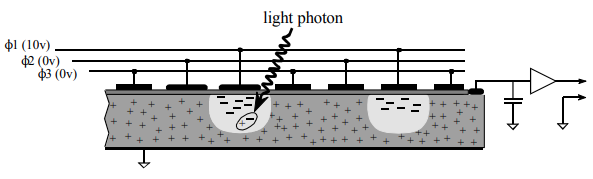
\includegraphics[width=0.4\textwidth]{ccd2.png}
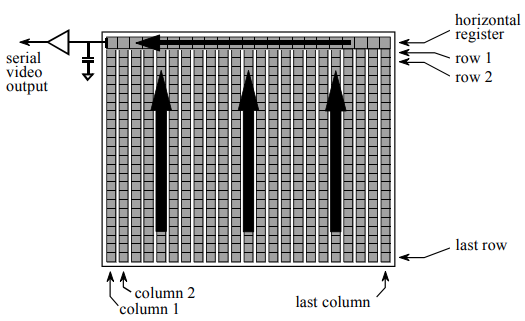
\includegraphics[width=0.35\textwidth]{ccd.png}
\caption{\label{fig:2} The readout scheme of a charge-coupled device (CCD) for capturing digital images.}
\end{figure}

\end{document}
